\chapter{Sources of Systematic Uncertainty}~\label{ch:systematics}
In this chapter we discuss the various sources of systematic uncertainties arising from limitations in the experimental setup as well as the modelling of both the signal and the background. These systematics together with the bin-by-bin statistical uncertainties are considered as nuisance parameters in the fit for the final limit setting. These uncertainties which affect either the shape or normalization of the distributions are summarized in Table~\ref{tab:Systematics}. 

\begin{table}[h]{\scriptsize{\caption{Systematic uncertanties and nuisances considered in non-resonant search.}
\label{tab:Systematics}\begin{center}\begin{tabular}{c|cccc}\hline
Name                  & Number of Nuisances         & Shape or Rate& On Signal(S) or BKG(B)&Constrained over SRs\\\hline
Signal strength       & 1                           & Rate         & S              & 6 SRs               \\ \hline
Luminosity            & 1                           & Rate (1.6\%) & S              & 6 SRs               \\
Normal. real \gmgm    & 6 uncorrelated              & Rate (5\%)   & B (\gmgm)      & 1 for each SR       \\
Normal. fake $\gj,~jj$& 6 uncorrelated              & Rate (30\%)  & B ($\gj,jj$)   & 1 for each SR       \\
kFactor QCD scales    & 2, each corr. across years  & Shape        & B (\gmgm)      & 1 for each of BB, BE\\
Photon efficiency     & 1 corr. across SRs          & Shape        & S \& B (\gmgm) & 6 SRs               \\
Energy scale gain     & 1 corr. across SRs          & Shape        & S \& B (\gmgm) & 6 SRs               \\
%Energy scale syst.    & 1 corr. across SRs          & Shape        & S \& B (\gmgm) & 6 SRs               \\
Energy scale sigma    & 1 corr. across SRs          & Shape        & S \& B (\gmgm) & 6 SRs               \\
Fake sample           & 6 corr. across SRs          & Shape        & B ($\gj,jj$)   & 1 for each SR       \\
kFactors stat.par.0-3 & 4 each corr. across SRs     & Shape        & B ($\gj,jj$)   & 6 SRs               \\
PDFs 1-50 hessians    & 50, each corr. across 6 SRs & Shape        & B (\gmgm)      & 6 SRs               \\
Pileup                & 1 corr. across SRs          & Shape        & S \& B (\gmgm) & 6 SRs               \\ \hline
\end{tabular}\end{center}
}\end{table}

The systematic uncertainties are treated introducing nuisance parameters. The first column of Table~\ref{tab:Systematics} show the names of these sources. The second column presents the number of nuisances together with the correlation information. The third column shows whether the nuisance parameter affects the overall normalization or the shape of the distributions, while the fourth column indicates whether the parameter is constrained for the signal, background or both. Finally, the fifth column shows which signal regions (SRs) the nuisance is constrained over. In this analysis, there is a total of 6 signal regions corressponding to BB, which are barrel-barrel events or BE, which are barrel-endcap events, for each of the three years: 2016, 2017, 2018.

%%%%%%%%%%%%%%%%%%%%%%%%%%%%%

% he addition of systematic uncertainties thus introduces
% auxiliary parameters into the likelihood, known as nuisance parameters (NPs), over
% which the likelihood will also need to be maximized in order to determine the best-fit
% signal strength. The likelihood function modified in this way is known as the profile
% likelihood and takes the form

% in~Section~\ref{sec:summary_syst}.

% \section{Summary of the Systematic Uncertainties} \label{sec:summary_syst}

% The various sources of systematic uncertainties which are considered are summarized in table \ref{tab:Systematics}.

% \subsection{Luminosity Uncertainty}~\label{subsec:lumi_uncertainty}

\section{Real Background Systematic Uncertainties}~\label{sec:realBKGSYS}
% In this section, we discuss more details on the systematic uncertainties associated with the real and fake background modelling. 
% \textbf{For Normalization}, 
Since the Real SM Prompt diphoton background was only performed at NNLO accuracy and higher order terms are unaccounted for, we allow the normalization of the background to float freely, constrained only by the data, at a rate of 5\%. This rate also absorbs the systematic uncertainties associated with the integrated luminosity measurement and inefficiencies from the trigger and high-$p_T$ photon ID selection. In total, six nuisances are assigned, one for each of the six signal regions. 
% This 5\% rate uncertainty is assigned as a prefit uncertainty with a lognormal prior.

Two sources of shape uncertainties on the SM background come from the variation of the K factor scales and the Parton Distribution Function (PDF) uncertainties. We account for the theoretical uncertainty in the factorization and renormalization in QCD scales. This uncertainty is determined by varying the scales used in the K factor calculation, separately for BB and BE. The renormalization and factorization scales are varied simultaneously by a factor of two in each direction, and taking the resultant variation as a measure of the systematic uncertainty on the k-factor. This is found to give an uncertainty varying from $^{+5.4}_{-4.3}$\% ($^{+4.1}_{-3.6}$\%) to $^{+7.3}_{-5.8}$\% ($^{+11.2}_{-6.9}$\%) for BB (BE) at 0.5\TeV and 2.0\TeV,
respectively. In \MCFM, these scales affect the differential cross-section calculations through the estimation of the truncation point of the perturbative calculation. Figure~\ref{Fig:sys_fs} shows the k-factor variations as well as the ratio of these variations over the default value or nominal value of $\mgg$. From these figures, we see that the uncertainty increases with increasing $\mgg$. 

The PDF uncertainties are obtained from a new feature from \MCFM~9.0 which allows us to use PDF weights to calculate uncertainties. \MCFM constructs a Hessian matrix which contains information about how variations in the parameters of the PDF model affect the goodness-of-fit to the experimental data, which is a way to estimate the uncertainties associated with the PDF. In particular, the PDF uncertainties on the real background \mgg are estimated using the \texttt{NNPDF30\_nnlo\_as\_0118\_hessian} PDF set. By construction, this PDF set has the same central values as the \texttt{NNPDF30\_nnlo\_as\_0118} set used in the \SHERPA MC samples and the \MCFM cross-section calculations with uncertainties provided by eigenvectors rather than PDF replicas. This procedure simplifies the inclusion of PDF uncertainties as the eigenvector variations are uncorrelated, in contrast with the standard PDF set. Fifty (50) eigenvectors are provided in the Hessian PDF set and these are shown in Figure~\ref{Fig:PDFs_Sys1} and Figure~\ref{Fig:PDFs_Sys2}. These plots are BB plots showing the resulting uncertainties from the 50 variations of the PDFs eigenvectors which refer to variations in the sets of PDFs obtained from global fits to experimental data. MCFM 9.0 allows the evaluation of uncertainties due to individual eigenvectors and in principle should allow for calculating uncertainties on the full NNLO cross section. In practice, we found that it was impossible to complete a significant number of the NNLO jobs within the maximum allowed CPU/wall clock time limits. These eigenvectors represent directions in the parameter space of the PDF model. Figure~\ref{Fig:sys_pdf} shows the uncertainty on the real background arising from the quadratic combination of all 50 individual variations. 
% Figure~\ref{Fig:sys_pdf} shows the evaluation of the PDF uncertainty bands (50 variations quadratically combined) for both the LO and NLO computations.
% The consistency between the results gives us confidence that the fully correct NNLO predicted uncertainties would be quite close to the NLO result, particularly for a subdominant uncertainty such as the PDF uncertainty.

% PDF Hessian Matrix: To quantify the uncertainties in PDFs, a Hessian matrix is constructed. This matrix contains information about how variations in the parameters of the PDF model affect the goodness-of-fit to the experimental data. It provides a way to estimate the uncertainties associated with the PDFs.

% Eigenvectors of the Hessian Matrix: The eigenvectors of the Hessian matrix represent directions in the parameter space of the PDF model. Each eigenvector corresponds to a specific variation or direction that contributes to the uncertainty in the PDFs. The eigenvalues associated with these eigenvectors quantify the magnitude of these variations.

The exact treatment of the PDFs uncertainties are described as follows. For each of the 50 eigenvector variations, a pair of different \mgg spectra is derived. These pairs correspond to $\pm1\simga$ variations of eigenvectors. A nuisance parameter with a gaussian prior pdf for each pair is assigned. Each of these is constrained simultaneously over all the six signal regions. We observe that the resulting shape uncertainties are small and affect less than 2\% the spectra for $\mgg<3.5\TeV$.

Uncertainties due to the photon energy scale and resolution shown in Figure~\ref{fig:E_scale_sys} have also been considered in the analysis. For each of these uncertainties, two different $\mgg$  shapes are formed (corresponding to the plus and minus shifts) for each of the six signal regions. We assign a single nuisance parameter for each which is constrained over all six SRs. For the ``energy scale statistical" and the ``energy sigma" there were neither shape nor rate effect in the variations and so these source of uncertainty has been omitted to preserve computing resources.
% Figure~\ref{fig:E_scale_sys} shows the systematic uncertainty trends of the ratio between the variation and the default. 

% \textbf{For photon energy scale and resolution}~\ref{fig:E_scale_sys}, we include the efficiency and the energy scale gains. 

\begin{figure}[!htbp]{ \centering{
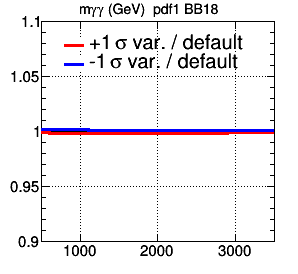
\includegraphics[width=0.16\textwidth]{fig/spectra__pdf1_BB18_ADDGRW.png}
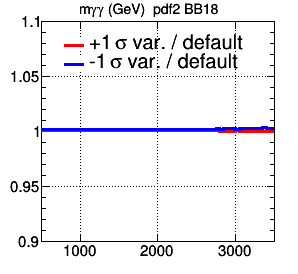
\includegraphics[width=0.16\textwidth]{fig/spectra__pdf2_BB18_ADDGRW.png}
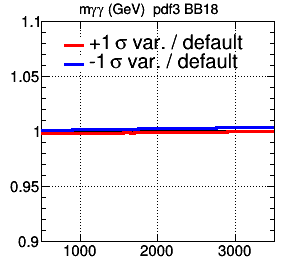
\includegraphics[width=0.16\textwidth]{fig/spectra__pdf3_BB18_ADDGRW.png}
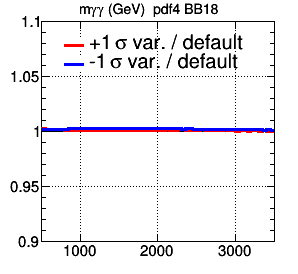
\includegraphics[width=0.16\textwidth]{fig/spectra__pdf4_BB18_ADDGRW.png}
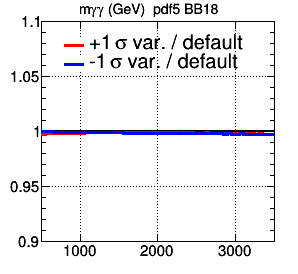
\includegraphics[width=0.16\textwidth]{fig/spectra__pdf5_BB18_ADDGRW.png}\\
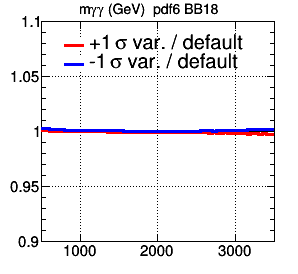
\includegraphics[width=0.16\textwidth]{fig/spectra__pdf6_BB18_ADDGRW.png}
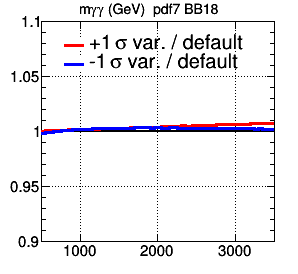
\includegraphics[width=0.16\textwidth]{fig/spectra__pdf7_BB18_ADDGRW.png}
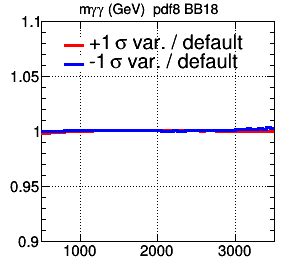
\includegraphics[width=0.16\textwidth]{fig/spectra__pdf8_BB18_ADDGRW.png}
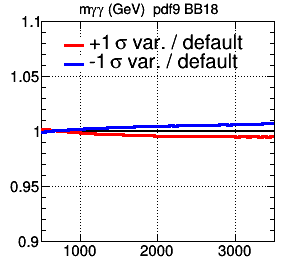
\includegraphics[width=0.16\textwidth]{fig/spectra__pdf9_BB18_ADDGRW.png}
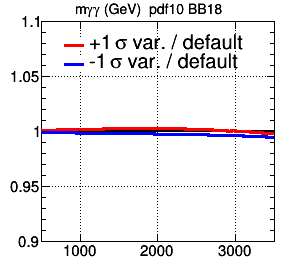
\includegraphics[width=0.16\textwidth]{fig/spectra__pdf10_BB18_ADDGRW.png}\\
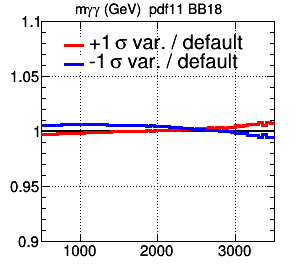
\includegraphics[width=0.16\textwidth]{fig/spectra__pdf11_BB18_ADDGRW.png}
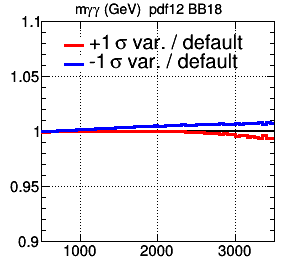
\includegraphics[width=0.16\textwidth]{fig/spectra__pdf12_BB18_ADDGRW.png}
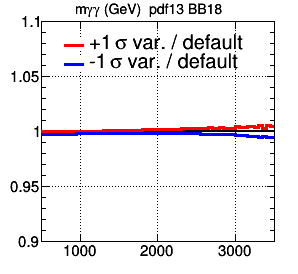
\includegraphics[width=0.16\textwidth]{fig/spectra__pdf13_BB18_ADDGRW.png}
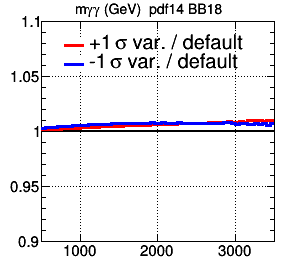
\includegraphics[width=0.16\textwidth]{fig/spectra__pdf14_BB18_ADDGRW.png}
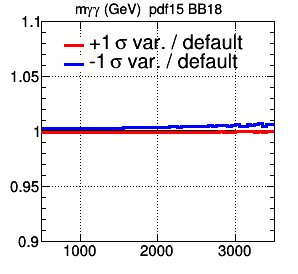
\includegraphics[width=0.16\textwidth]{fig/spectra__pdf15_BB18_ADDGRW.png}\\
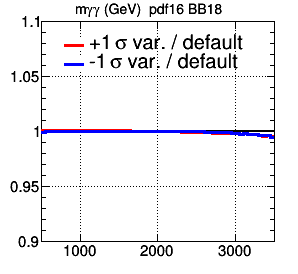
\includegraphics[width=0.16\textwidth]{fig/spectra__pdf16_BB18_ADDGRW.png}
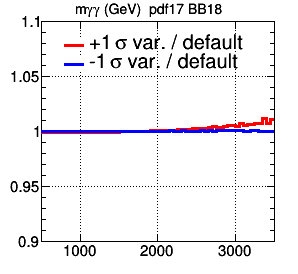
\includegraphics[width=0.16\textwidth]{fig/spectra__pdf17_BB18_ADDGRW.png}
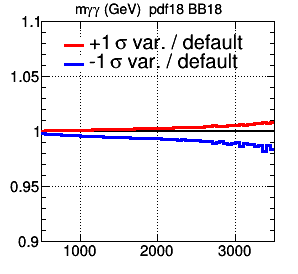
\includegraphics[width=0.16\textwidth]{fig/spectra__pdf18_BB18_ADDGRW.png}
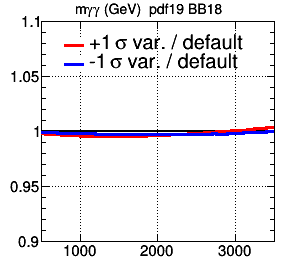
\includegraphics[width=0.16\textwidth]{fig/spectra__pdf19_BB18_ADDGRW.png}
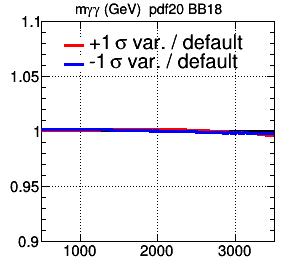
\includegraphics[width=0.16\textwidth]{fig/spectra__pdf20_BB18_ADDGRW.png}\\
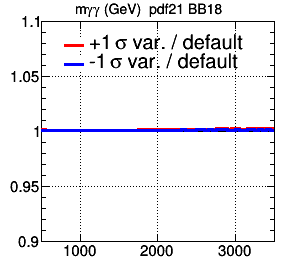
\includegraphics[width=0.16\textwidth]{fig/spectra__pdf21_BB18_ADDGRW.png}
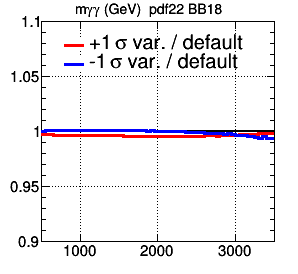
\includegraphics[width=0.16\textwidth]{fig/spectra__pdf22_BB18_ADDGRW.png}
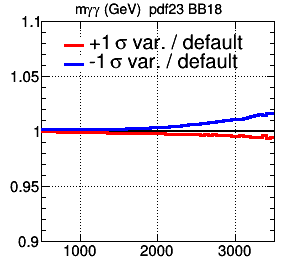
\includegraphics[width=0.16\textwidth]{fig/spectra__pdf23_BB18_ADDGRW.png}
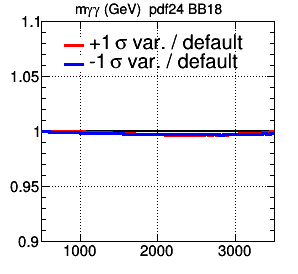
\includegraphics[width=0.16\textwidth]{fig/spectra__pdf24_BB18_ADDGRW.png}
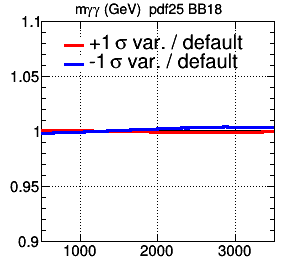
\includegraphics[width=0.16\textwidth]{fig/spectra__pdf25_BB18_ADDGRW.png}\\


% 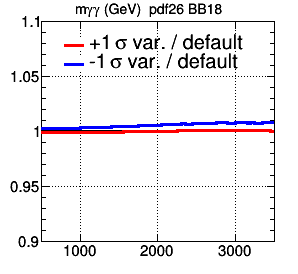
\includegraphics[width=0.16\textwidth]{fig/spectra__pdf26_BB18_ADDGRW.png}
% 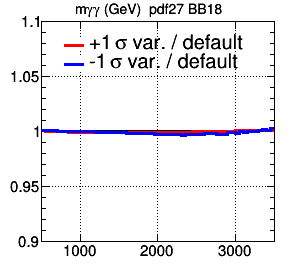
\includegraphics[width=0.16\textwidth]{fig/spectra__pdf27_BB18_ADDGRW.png}
% 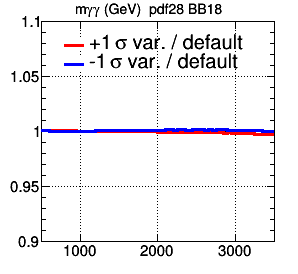
\includegraphics[width=0.16\textwidth]{fig/spectra__pdf28_BB18_ADDGRW.png}
% 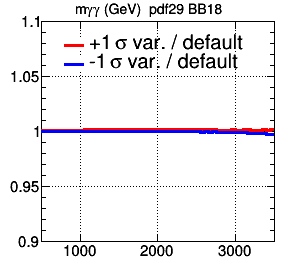
\includegraphics[width=0.16\textwidth]{fig/spectra__pdf29_BB18_ADDGRW.png}
% 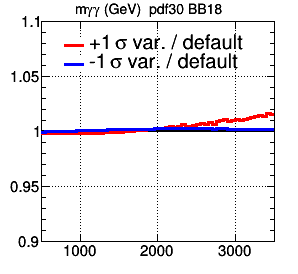
\includegraphics[width=0.16\textwidth]{fig/spectra__pdf30_BB18_ADDGRW.png}\\
% 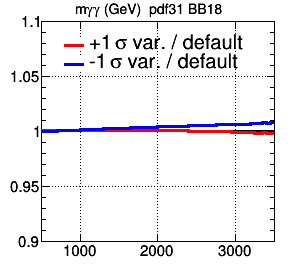
\includegraphics[width=0.16\textwidth]{fig/spectra__pdf31_BB18_ADDGRW.png}
% 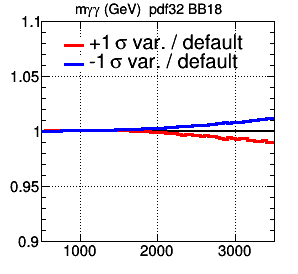
\includegraphics[width=0.16\textwidth]{fig/spectra__pdf32_BB18_ADDGRW.png}
% 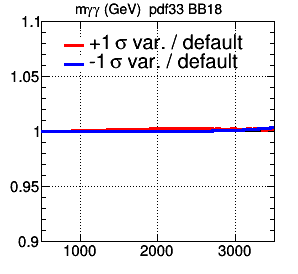
\includegraphics[width=0.16\textwidth]{fig/spectra__pdf33_BB18_ADDGRW.png}
% 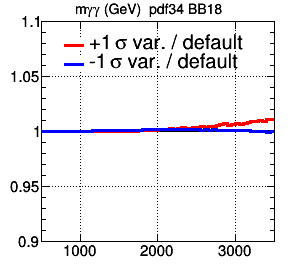
\includegraphics[width=0.16\textwidth]{fig/spectra__pdf34_BB18_ADDGRW.png}
% 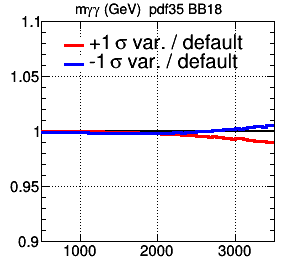
\includegraphics[width=0.16\textwidth]{fig/spectra__pdf35_BB18_ADDGRW.png}\\
% 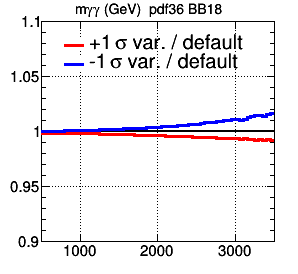
\includegraphics[width=0.16\textwidth]{fig/spectra__pdf36_BB18_ADDGRW.png}
% 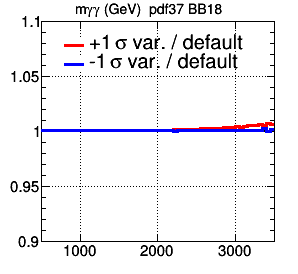
\includegraphics[width=0.16\textwidth]{fig/spectra__pdf37_BB18_ADDGRW.png}
% 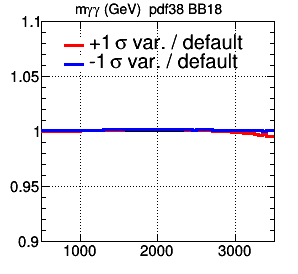
\includegraphics[width=0.16\textwidth]{fig/spectra__pdf38_BB18_ADDGRW.png}
% 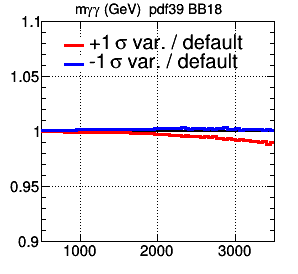
\includegraphics[width=0.16\textwidth]{fig/spectra__pdf39_BB18_ADDGRW.png}
% 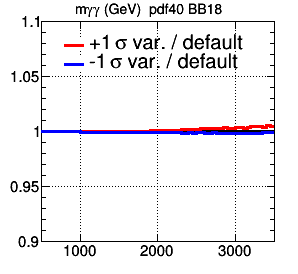
\includegraphics[width=0.16\textwidth]{fig/spectra__pdf40_BB18_ADDGRW.png}\\
% 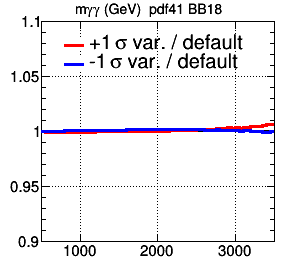
\includegraphics[width=0.16\textwidth]{fig/spectra__pdf41_BB18_ADDGRW.png}
% 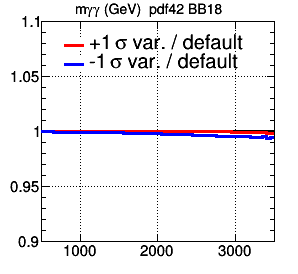
\includegraphics[width=0.16\textwidth]{fig/spectra__pdf42_BB18_ADDGRW.png}
% 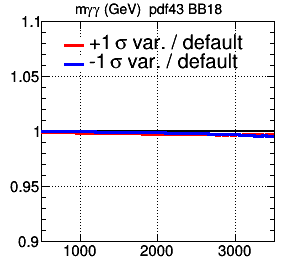
\includegraphics[width=0.16\textwidth]{fig/spectra__pdf43_BB18_ADDGRW.png}
% 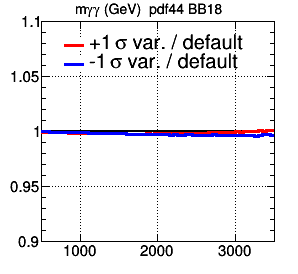
\includegraphics[width=0.16\textwidth]{fig/spectra__pdf44_BB18_ADDGRW.png}
% 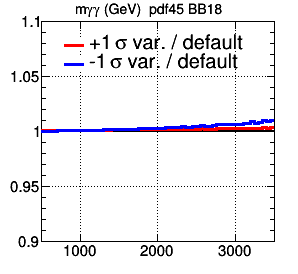
\includegraphics[width=0.16\textwidth]{fig/spectra__pdf45_BB18_ADDGRW.png}\\
% 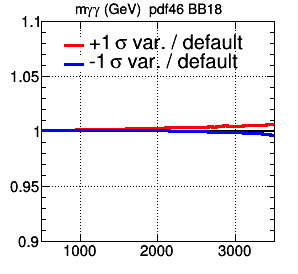
\includegraphics[width=0.16\textwidth]{fig/spectra__pdf46_BB18_ADDGRW.png}
% 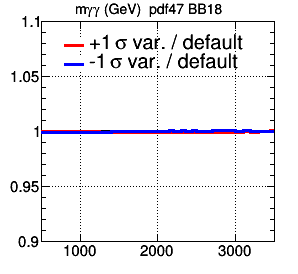
\includegraphics[width=0.16\textwidth]{fig/spectra__pdf47_BB18_ADDGRW.png}
% 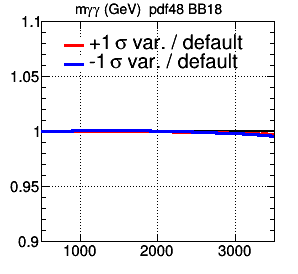
\includegraphics[width=0.16\textwidth]{fig/spectra__pdf48_BB18_ADDGRW.png}
% 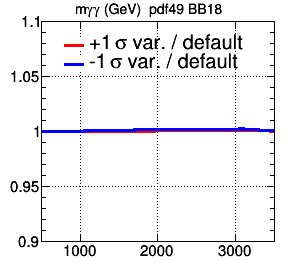
\includegraphics[width=0.16\textwidth]{fig/spectra__pdf49_BB18_ADDGRW.png}
% 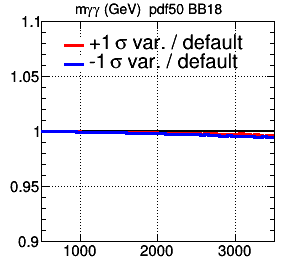
\includegraphics[width=0.16\textwidth]{fig/spectra__pdf50_BB18_ADDGRW.png}\\}
\caption{The resulting uncertainties from first 25 of the 50 variations of the PDFs eigenvectors. 
The variation over central estimate is shown versus the \mgg. 
(Plots shown stand for BB, while the corresponding for BE, as they are very similar, have been omitted).
} 
\label{Fig:PDFs_Sys1} }
\end{figure}

\begin{figure}[!htbp]{ \centering{
% \includegraphics[width=0.16\textwidth]{fig/spectra__pdf1_BB18_ADDGRW.png}
% \includegraphics[width=0.16\textwidth]{fig/spectra__pdf2_BB18_ADDGRW.png}
% \includegraphics[width=0.16\textwidth]{fig/spectra__pdf3_BB18_ADDGRW.png}
% \includegraphics[width=0.16\textwidth]{fig/spectra__pdf4_BB18_ADDGRW.png}
% \includegraphics[width=0.16\textwidth]{fig/spectra__pdf5_BB18_ADDGRW.png}\\
% \includegraphics[width=0.16\textwidth]{fig/spectra__pdf6_BB18_ADDGRW.png}
% \includegraphics[width=0.16\textwidth]{fig/spectra__pdf7_BB18_ADDGRW.png}
% \includegraphics[width=0.16\textwidth]{fig/spectra__pdf8_BB18_ADDGRW.png}
% \includegraphics[width=0.16\textwidth]{fig/spectra__pdf9_BB18_ADDGRW.png}
% \includegraphics[width=0.16\textwidth]{fig/spectra__pdf10_BB18_ADDGRW.png}\\
% \includegraphics[width=0.16\textwidth]{fig/spectra__pdf11_BB18_ADDGRW.png}
% \includegraphics[width=0.16\textwidth]{fig/spectra__pdf12_BB18_ADDGRW.png}
% \includegraphics[width=0.16\textwidth]{fig/spectra__pdf13_BB18_ADDGRW.png}
% \includegraphics[width=0.16\textwidth]{fig/spectra__pdf14_BB18_ADDGRW.png}
% \includegraphics[width=0.16\textwidth]{fig/spectra__pdf15_BB18_ADDGRW.png}\\
% \includegraphics[width=0.16\textwidth]{fig/spectra__pdf16_BB18_ADDGRW.png}
% \includegraphics[width=0.16\textwidth]{fig/spectra__pdf17_BB18_ADDGRW.png}
% \includegraphics[width=0.16\textwidth]{fig/spectra__pdf18_BB18_ADDGRW.png}
% \includegraphics[width=0.16\textwidth]{fig/spectra__pdf19_BB18_ADDGRW.png}
% \includegraphics[width=0.16\textwidth]{fig/spectra__pdf20_BB18_ADDGRW.png}\\
% \includegraphics[width=0.16\textwidth]{fig/spectra__pdf21_BB18_ADDGRW.png}
% \includegraphics[width=0.16\textwidth]{fig/spectra__pdf22_BB18_ADDGRW.png}
% \includegraphics[width=0.16\textwidth]{fig/spectra__pdf23_BB18_ADDGRW.png}
% \includegraphics[width=0.16\textwidth]{fig/spectra__pdf24_BB18_ADDGRW.png}
% \includegraphics[width=0.16\textwidth]{fig/spectra__pdf25_BB18_ADDGRW.png}\\




\includegraphics[width=0.16\textwidth]{fig/spectra__pdf26_BB18_ADDGRW.png}
\includegraphics[width=0.16\textwidth]{fig/spectra__pdf27_BB18_ADDGRW.png}
\includegraphics[width=0.16\textwidth]{fig/spectra__pdf28_BB18_ADDGRW.png}
\includegraphics[width=0.16\textwidth]{fig/spectra__pdf29_BB18_ADDGRW.png}
\includegraphics[width=0.16\textwidth]{fig/spectra__pdf30_BB18_ADDGRW.png}\\
\includegraphics[width=0.16\textwidth]{fig/spectra__pdf31_BB18_ADDGRW.png}
\includegraphics[width=0.16\textwidth]{fig/spectra__pdf32_BB18_ADDGRW.png}
\includegraphics[width=0.16\textwidth]{fig/spectra__pdf33_BB18_ADDGRW.png}
\includegraphics[width=0.16\textwidth]{fig/spectra__pdf34_BB18_ADDGRW.png}
\includegraphics[width=0.16\textwidth]{fig/spectra__pdf35_BB18_ADDGRW.png}\\
\includegraphics[width=0.16\textwidth]{fig/spectra__pdf36_BB18_ADDGRW.png}
\includegraphics[width=0.16\textwidth]{fig/spectra__pdf37_BB18_ADDGRW.png}
\includegraphics[width=0.16\textwidth]{fig/spectra__pdf38_BB18_ADDGRW.png}
\includegraphics[width=0.16\textwidth]{fig/spectra__pdf39_BB18_ADDGRW.png}
\includegraphics[width=0.16\textwidth]{fig/spectra__pdf40_BB18_ADDGRW.png}\\
\includegraphics[width=0.16\textwidth]{fig/spectra__pdf41_BB18_ADDGRW.png}
\includegraphics[width=0.16\textwidth]{fig/spectra__pdf42_BB18_ADDGRW.png}
\includegraphics[width=0.16\textwidth]{fig/spectra__pdf43_BB18_ADDGRW.png}
\includegraphics[width=0.16\textwidth]{fig/spectra__pdf44_BB18_ADDGRW.png}
\includegraphics[width=0.16\textwidth]{fig/spectra__pdf45_BB18_ADDGRW.png}\\
\includegraphics[width=0.16\textwidth]{fig/spectra__pdf46_BB18_ADDGRW.png}
\includegraphics[width=0.16\textwidth]{fig/spectra__pdf47_BB18_ADDGRW.png}
\includegraphics[width=0.16\textwidth]{fig/spectra__pdf48_BB18_ADDGRW.png}
\includegraphics[width=0.16\textwidth]{fig/spectra__pdf49_BB18_ADDGRW.png}
\includegraphics[width=0.16\textwidth]{fig/spectra__pdf50_BB18_ADDGRW.png}\\}
\caption{The resulting uncertainties from the last 25 of 50 variations of the PDFs eigenvectors. 
The variation over central estimate is shown versus the \mgg. 
(Plots shown stand for BB, while the corresponding for BE, as they are very similar, have been omitted).
} 
\label{Fig:PDFs_Sys2} }
\end{figure}

\section{Fake Background Systematic Uncertainties}~\label{sec:fakeBKGSYS}
We assign a 30\% systematic uncertainty to the normalization of the fake $gj$ background covering the degree of variation in the fake rate in bins of photon $\eta$, number of primary vertices, pileup, and the choice of the sideband definition and template variable. Six different nuisances have been assigned, one for each of the six signal regions, with a 30\% magnitude and a lognormal prior. Figure~\ref{fig:FakeSampleSys} shows the effect of the "fake sample" systematic uncertainty listed in Table~\ref{tab:Systematics}. We've decided to drop the jj contribution since it is 2 orders of magnitude smaller than the gj contribution. The 30\% rate also covers the non-closure seen in the fake rate closure test, and the differences between the fake rate derived from the jet-triggered and muon-triggered data samples. The jet-triggered and the muon-triggered data samples resulted in slightly different fake rate estimates and the mean of the two was taken as the central value for the fake rate estimate. The maximum and minimum extremes were used to assign two (plus and minus) alternative predictions for the fake background. This source of uncertainty accounts for the difference in the quark and gluon contents of the two data sets. The details of these studies are found in Sec.~\ref{sec:bkg_fake} and Sec.~\ref{sec:closure_test}. 

\section{Signal Systematic Uncertainties}~\label{sec:sigSYS}
The signal distributions are normalized to the integrated luminosity. We assign a rate of 1.6\% systematic uncertainty related to the uncertainties in the measurement of the integrated luminosity. The photon selection efficiency, energy scale and resolution, as well as the effect of pileup have been considered as shape-based uncertainties. 
%%%%%%%%%%%%%%%%%%%%%%%%%%%%%



% \textbf{For photon energy scale and resolution}~\ref{fig:E_scale_sys}, we include the efficiency and the energy scale gains. 

% Systematic uncertainties are assigned to the normalization of the signal calculation to account
% for the uncertainties in measurements of the integrated luminosity and overall diphoton
% selection efficiency, corresponding to 2.5% [83] and 6%, respectively. The selection efficiency
% includes the trigger and high-pT photon ID efficiency, which are 3% per photon. The PDF
% uncertainties affecting the signal shape are determined using the same procedure as is done for
% the background, by separately varying the 26 eigenvalue pairs using diphox at NLO. These
% PDF uncertainties are assumed to be 100% correlated between the signal and background.
% The effect of the PDF uncertainty on the signal cross section is considered a theoretical
% uncertainty and not treated as a systematic uncertainty.


%%%%%%%%%%%%%%%%%%%%%%%%%%%%%





% \textbf{For photon energy scale and resolution}~\ref{fig:E_scale_sys} there are four sources of systematic uncertainty:
% \begin{itemize}
% \item efficiency
% \item energy scale gain
% \textcolor{gray}{
% \item energy scale systematic (found negligible and we currently dropped it) 
% \item energy scale statistical (found negligible and we currently dropped it)
% \item energy sigma (found negligible and we currently dropped it)
% }
% \end{itemize}

% \FIXME{What led us to the conclusion that this is negligible.}



% The differences in \mgg shapes and rate which the above variations lead are presented in Figure \ref{fig:E_scale_sys}.
% Columns present the three residual sources of uncertainty, while rows list the six SRs. A single nuisance is attribute for each column.


% The resulting effect on the fake background $\gj,jj$ can bee seen in Figure \ref{fig:FakeSampleSys} in which the ratio of each variation over central prediction is plotted as a function of \mgg mass.
% The spectra are populated up to $\mgg\sim 1.5 \TeV$ (and fluctuates above that) due to low statistics as fake background is mostly at low \mgg. A single nuisance parameter is assigned for this source for each one of the six SRs



% Figure \ref{Fig:PDFs_Sys} present the individual trends (in the from of $\pm$variation over central estimate) each of variations lead to as a function of \mgg.

% \textbf{For the pileup}, systematic uncertainty is assigned scaling the minimum bias cross section ( 69.2 mb) by $\pm4.6\%$.



% \section{Real and Fake Background Systematic Uncertainties}

\begin{figure}[!htbp]{ \centering{
\includegraphics[width=0.45\textwidth]{fig/pdf_uncertainty_band_LO.pdf}% generated by pdf_uncertainty.exe
\includegraphics[width=0.45\textwidth]{fig/pdf_uncertainty_band_nlo.pdf} }
\caption{The uncertainty on the real \gmgm background that arises from PDFs (parton distribution function) uncertainties, displayed separately for the barrel-barrel and barrel-endcap regions, for evaluations at LO (left) and NLO (right).} 
\label{Fig:sys_pdf} }
\end{figure}

% - Normal. real \gmgm    & 6 uncorrelated              & Rate (5\%)   & B (\gmgm)      & 1 for each SR  
% Normal. fake $\gj,~jj$& 6 uncorrelated              & Rate (30\%)  & B ($\gj,jj$)   & 1 for each SR    
% kFactor QCD scales    & 2, each corr. across years  & Shape        & B (\gmgm)      & 1 for each of BB, BE\\
% Photon efficiency     & 1 corr. across SRs          & Shape        & S \& B (\gmgm) & 6 SRs               \\
% Energy scale gain     & 1 corr. across SRs          & Shape        & S \& B (\gmgm) & 6 SRs               \\
% Energy scale sigma    & 1 corr. across SRs          & Shape        & S \& B (\gmgm) & 6 SRs               \\
% Energy scale sigma    & 1 corr. across SRs          & Shape        & S \& B (\gmgm) & 6 SRs               \\
% Fake sample           & 6 corr. across SRs          & Shape        & B ($\gj,jj$)   & 1 for each SR       \\
% kFactors stat.par.0-3 & 4 each corr. across SRs     & Shape        & B ($\gj,jj$)   & 6 SRs               \\
% PDFs 1-50 hessians    & 50, each corr. across 6 SRs & Shape        & B (\gmgm)      & 6 SRs               \\
% Pileup                & 1 corr. across SRs          & Shape        & S \& B (\gmgm) & 6 SRs               \\ \hline

\begin{figure}[!htbp]{ \centering{
\includegraphics[width=0.4\linewidth]{fig/kfactorScaleVariations_BB_preliminary_NNPDF.pdf} %generated by kfactorScaleVariations.exe
\includegraphics[width=0.4\linewidth]{fig/kfactorScaleVariations_BE_preliminary_NNPDF.pdf}
\includegraphics[width=0.4\linewidth]{fig/spectra__diphotonkfactorScalesBB_BB18_ADDGRW.png}
\includegraphics[width=0.4\linewidth]{fig/spectra__diphotonkfactorScalesBE_BE18_ADDGRW.png} }
\caption{Top: the NNLO (MCFM) k-factors for different factorization and renormalization (QCD) scales.
Bottom: the ratio of these variations over the central value as a function of \mgg.
Plots for the BB (barrel-barrel) on the left, and BE (barrel-endcap) on the right.}\label{Fig:sys_fs}
}\end{figure}

\begin{figure}[!htbp]{ \centering{
\includegraphics[width=0.32\linewidth]{fig/spectra__fakesample_BB16_ADDGRW.png}
\includegraphics[width=0.32\linewidth]{fig/spectra__fakesample_BB17_ADDGRW.png}
\includegraphics[width=0.32\linewidth]{fig/spectra__fakesample_BB18_ADDGRW.png}
\includegraphics[width=0.32\linewidth]{fig/spectra__fakesample_BE16_ADDGRW.png}
\includegraphics[width=0.32\linewidth]{fig/spectra__fakesample_BE17_ADDGRW.png}
\includegraphics[width=0.32\linewidth]{fig/spectra__fakesample_BE18_ADDGRW.png} }
\caption{The effect of ``fake sample" systematic uncertainty over the fake background $\gj,jj$ vs the \mgg spectra. Top (bottom) the BB (BE) channels, left to right for years 2016, 2017, and 2018 respectively.
} \label{fig:FakeSampleSys}
}\end{figure}


% \section{Signal Systematic Uncertainties}

\begin{figure}[!htbp]
\centering
\includegraphics[width=0.24\linewidth, height=1in]{fig/spectra__eff_BB16_ADDGRW.png}
\includegraphics[width=0.24\linewidth, height=1in]{fig/spectra__energyScaleGain_BB16_ADDGRW.png}\\
\includegraphics[width=0.24\linewidth, height=1in]{fig/spectra__eff_BE16_ADDGRW.png}
\includegraphics[width=0.24\linewidth, height=1in]{fig/spectra__energyScaleGain_BE16_ADDGRW.png}\\
\includegraphics[width=0.24\linewidth, height=1in]{fig/spectra__eff_BB17_ADDGRW.png}
\includegraphics[width=0.24\linewidth, height=1in]{fig/spectra__energyScaleGain_BB17_ADDGRW.png}\\
\includegraphics[width=0.24\linewidth, height=1in]{fig/spectra__eff_BE17_ADDGRW.png}
\includegraphics[width=0.24\linewidth, height=1in]{fig/spectra__energyScaleGain_BE17_ADDGRW.png}\\
\includegraphics[width=0.24\linewidth, height=1in]{fig/spectra__eff_BB18_ADDGRW.png}
\includegraphics[width=0.24\linewidth, height=1in]{fig/spectra__energyScaleGain_BB18_ADDGRW.png}\\
\includegraphics[width=0.24\linewidth, height=1in]{fig/spectra__eff_BE18_ADDGRW.png}
\includegraphics[width=0.24\linewidth, height=1in]{fig/spectra__energyScaleGain_BE18_ADDGRW.png}
\caption{The left shows the systematic uncertainty trends of ``variation/central" ratios of real \gmgm background vs \mgg for the sources of: ``efficiency", and right for ``energy scale gain". Top to bottom: the six SRs of BB16, ..., BE18 respectively.}
\label{fig:E_scale_sys}
\end{figure}







\newpage
% \section{References}
% \renewcommand{\bibsection}{}%removes the spaces and unwanted references heading from the list
% \begin{singlespacing}
% \bibliographystyle{apsrev}
% \bibliography{Ref_Systematics.bib}
% \end{singlespacing}\par